% RSS paper_template.tex from the course/Downloads uses IEEEtran.cls in conference mode.
\documentclass[conference]{IEEEtran}
\usepackage{times}
\usepackage[numbers]{natbib}
\usepackage{booktabs}
\usepackage{amsmath}
\usepackage{graphicx}
\usepackage{array}
\usepackage{xcolor}
\usepackage{tabularx}
\usepackage{CJKutf8}
\usepackage[bookmarks=true]{hyperref}

\pdfinfo{
   /Author (Zehui Liu; Sijie Chen)
   /Title  (Physics-Aware Music-to-Humanoid Dance Retargeting in MuJoCo)
   /Subject (Robotics, robot learning, humanoid motion retargeting)
   /Keywords (Humanoid robot; dance generation; retargeting; MuJoCo; Unitree G1)
}

\begin{document}
\begin{CJK*}{UTF8}{gbsn}

\title{Physics-Aware Music-to-Humanoid Dance Retargeting in MuJoCo}

\author{\IEEEauthorblockN{刘泽辉 (524531910022) \quad 陈思洁 (524531910025)}
\IEEEauthorblockA{Intelligent Robotics Final Project Midterm Report}}

\maketitle

\begin{abstract}
This project studies how music-conditioned human dance can be adapted into physically feasible motions for a simulated humanoid robot. The original proposal planned an end-to-end pipeline from music input to robot dance execution using EDGE, motion retargeting, and MuJoCo physics simulation. At the midterm stage, we have implemented this pipeline for a Unitree G1 model and refined the problem formulation based on early failures: visually plausible human dance is often not dynamically feasible for a floating-base biped. Our current system includes EDGE-based dance generation, SMPL-to-G1 retargeting, IK-based arm adaptation, offline joint and root constraints, PD tracking in MuJoCo, and a robot-feasibility optimization layer. On a 10-second pop-style clip, the offline-filtered reference falls after 1.62 seconds, while a conservative balance-safe reference and the proposed feasibility-optimized reference both remain stable for the full rollout. The feasibility-optimized reference preserves more than three times the actuated motion amplitude of the conservative baseline, showing progress toward the stability--expressiveness trade-off in humanoid dance retargeting.
\end{abstract}

\IEEEpeerreviewmaketitle

\section{Problem Statement and Motivation}
The project asks whether a music-conditioned human dance generator can be connected to a physically simulated humanoid robot in a way that preserves dance expressiveness while satisfying robot constraints. This is meaningful because current dance generation models can synthesize visually convincing human motion, but animation quality alone does not imply robot executability. A humanoid robot must maintain balance, respect joint limits, avoid unrealistic accelerations, and track references through actuated joints under gravity.

Compared with the original proposal, the project scope has been refined but not changed in direction. The proposal specified three stages: EDGE-based music-to-dance generation, SMPL-to-humanoid retargeting, and MuJoCo simulation with PD control plus a possible PHC-style extension. We have kept this end-to-end objective, but our emphasis has shifted from simply producing a music-driven robot dance video to studying physics-aware retargeting and evaluation. The reason is empirical: direct retargeting from visually plausible human dance to the G1 often falls in unpinned simulation even when pinned-root playback looks acceptable. The current contribution is therefore an implemented pipeline, a diagnosis of the predicted stability risk, and a feasibility optimizer that searches for robot-friendly motion parameters.

\section{Related Work}
Music-conditioned dance generation provides the motion source for this project. AIST++ introduced paired music and 3D dance data for music-conditioned dance generation \cite{li2021aistpp}. Bailando uses a VQ-VAE and actor-critic GPT framework to generate dances with choreographic memory \cite{siyao2022bailando}. EDGE, which we use as the generator, is a diffusion-based editable dance generation model conditioned on music features \cite{tseng2023edge}. Later datasets and models such as FineDance and Lodge further improve full-body and long-horizon dance generation \cite{li2023finedance,li2024lodge}. These methods focus on kinematic dance quality rather than physical execution on a specific robot.

Humanoid simulation and tracking provide the robotics context. SMPL is the human body representation underlying many motion pipelines \cite{loper2015smpl}, and SMPLSim provides tools for simulating SMPL-shaped humanoids \cite{luo2024smplsim}. PHC demonstrates robust RL-based tracking of diverse human motion on simulated humanoids \cite{luo2023phc}. GMR addresses cross-embodiment retargeting to robots such as Unitree H1/G1 \cite{araujo2026gmr}. Our midterm baseline is simpler than PHC or GMR: direct SMPL-to-G1 retargeting followed by PD tracking in MuJoCo \cite{todorov2012mujoco} using the G1 model from MuJoCo Menagerie \cite{mujocomenagerie}. The project contribution is not a new dance generator or a new RL controller, but an application pipeline and feasibility analysis for generated dance on a robot body.

\section{Technical Approach}
The implemented system follows the original three-stage plan but adds explicit feasibility optimization. First, EDGE generates a 30 Hz SMPL-format dance sequence from a 10-second pop-style audio clip. Second, the sequence is retargeted to the G1 model. The initial v1 retargeting maps SMPL joint rotations to G1 lower-body, waist, and approximate arm joints through coordinate conversion from EDGE's human frame to MuJoCo's $z$-up frame. The v2 retargeting keeps the lower-body mapping but improves the arms with inverse kinematics: SMPL forward kinematics produces target upper-arm and forearm directions, each target upper-arm direction is transformed into the local G1 shoulder frame, shoulder pitch/roll are solved as a 2-DoF pointing problem, and the elbow angle is set from the upper-arm--forearm angle.

Third, the robot reference is processed by offline constraints and evaluated in MuJoCo. The offline pass smooths joints, clips joint ranges, limits per-frame rates and accelerations, stabilizes the floating root, and reduces foot slip in detected contact segments. The joint profiles are body-part dependent: wrist motion is heavily damped, shoulder and elbow motion are smoothed but preserved for visual expressiveness, waist motion is reduced, and hip/knee/ankle motion is kept conservative because it strongly affects balance. The PD tracker uses MuJoCo position actuators for the 29 actuated G1 joints, interpolates references at the simulator step size of 0.002 s, and declares a fall when pelvis height drops below 0.35 m.

The robot-feasibility optimizer searches over body-group gains
\begin{equation}
\theta=(g_{\rm leg},g_{\rm arm},g_{\rm waist},g_{xy},g_{\psi},g_z,s),
\end{equation}
where the gains control lower-body, upper-body, waist, root translation, root yaw, vertical motion, and smoothing strength. For each candidate $q_\theta(t)$, an unpinned MuJoCo rollout computes stability rate $r_{\rm stab}$, minimum pelvis height $h_{\min}$, mean tracking error $e_{\rm track}$, and a weighted motion amplitude score $m(q_\theta)$. The optimizer minimizes
\begin{align}
J(\theta)={}&w_f(1-r_{\rm stab})+w_h[h^*_{\min}-h_{\min}]_+ \nonumber\\
&+w_e e_{\rm track}-w_m m(q_\theta),
\end{align}
selecting the lowest-cost reference from safe presets and random samples. This is a lightweight rollout search rather than full trajectory optimization, but it directly addresses the main midterm failure mode.

\begin{table}[t]
\centering
\caption{Midterm response to the original proposal.}
\label{tab:proposal-response}
\setlength{\tabcolsep}{3pt}
\begin{tabularx}{\linewidth}{p{0.33\linewidth}X}
\toprule
Proposal item & Midterm status \\
\midrule
EDGE generation & Implemented for a pop-style clip with cached music features. \\
SMPL-to-G1 retargeting & Implemented custom G1 mapping and v2 arm IK. \\
PD control first & Implemented for pinned visualization and unpinned rollout. \\
Robot-fall risk & Confirmed; direct/filtered motions fall early. \\
Motion-scaling backup & Extended into rollout-based feasibility search. \\
PHC/RL extension & Deferred; reference feasibility is the current bottleneck. \\
Multi-genre evaluation & Deferred to final; current midterm uses one clip. \\
\bottomrule
\end{tabularx}
\end{table}

\section{Implementation Progress}
The current codebase covers the first four timeline phases from the proposal: environment setup, EDGE dance generation, G1 retargeting with simulation playback, and PD-based stability experiments. It also implements additional optimization stages that were not fully specified in the proposal: offline physical filtering, rollout candidate search, a conservative balance-safe fallback, and the robot-feasibility optimizer. The system produces both pinned-root showcase videos, which isolate joint-level visual tracking, and unpinned rollouts, which test whether the robot can remain standing under gravity.

\section{Preliminary Experiments and Results}
The preliminary experiment uses a 10-second pop-style audio clip. The generated human dance has beat alignment score 0.6866 with 9 detected music beats and 62 motion beats, computed using the EDGE-style acceleration-peak metric. The raw SMPL-to-G1 retargeting has a joint-limit boundary violation proxy of 0.69\% and only 11.8\% physical stability under direct PD tracking, falling at 1.18 s. These diagnostics support the proposal's concern that generated dances can be musically plausible but physically fragile.

We then compare three robot references in unpinned MuJoCo simulation: the offline-filtered reference, a conservative balance-safe reference, and the feasibility-optimized reference. Table~\ref{tab:results} reports stability rate, fall time, mean actuated joint tracking error, and mean actuated joint motion amplitude. Figure~\ref{fig:stability} plots pelvis height over time and shows that the offline-filtered reference crosses the fall threshold early, while the two safer references remain upright for the full rollout.

\begin{table}[t]
\centering
\caption{Unpinned MuJoCo rollout results on the 10-second pop-style clip. Higher stability and amplitude are better; lower tracking error is better.}
\label{tab:results}
\setlength{\tabcolsep}{3pt}
\begin{tabular}{lcccc}
\toprule
Method & Stab. & Fall & Err. & Amp. \\
\midrule
Offline-filtered & 16.2\% & 1.62s & 0.0108 & 0.0798 \\
Balance-safe & 100.0\% & none & 0.0034 & 0.0143 \\
Feasibility-opt. & 100.0\% & none & 0.0065 & 0.0516 \\
\bottomrule
\end{tabular}
\end{table}

\begin{figure}[t]
\centering
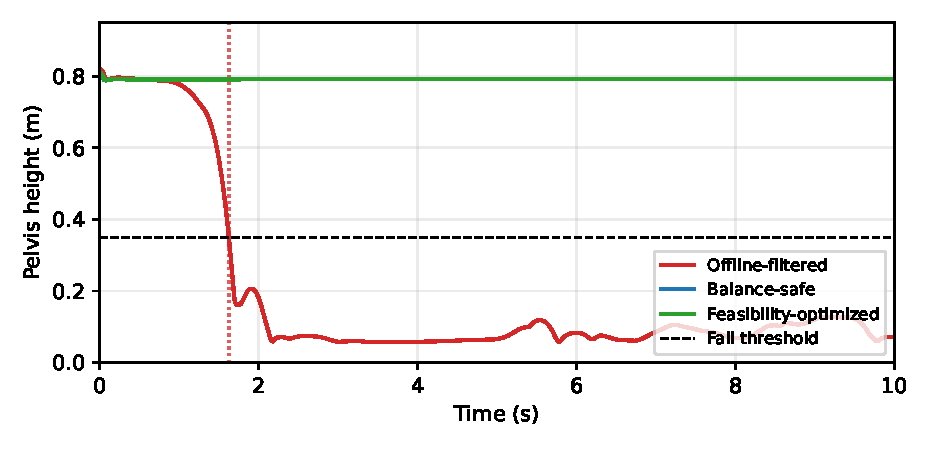
\includegraphics[width=\linewidth]{figures/stability_curve.pdf}
\caption{Pelvis height during unpinned MuJoCo rollouts. The offline-filtered reference falls early, while the balance-safe and feasibility-optimized references remain above the fall threshold for 10 s.}
\label{fig:stability}
\end{figure}

The feasibility-optimized motion remains stable for the full rollout while preserving more than three times the actuated motion amplitude of the balance-safe reference. However, it is still less expressive than pinned-root showcase playback, which confirms that the central challenge is not simply increasing amplitude but coordinating support, center of mass, and contact timing.

\section{Remaining Plan}
The next phase will complete the evaluation commitments from the proposal while improving the stability--expressiveness trade-off. First, the contact heuristic will be upgraded into a support-phase detector that separates double-support, left-support, right-support, and flight-like frames. Second, the feasibility optimizer will add center-of-mass and support-polygon terms so that lower-body motion can be increased only when the predicted support state can sustain it. Third, the evaluation will be expanded from one pop-style example to several clips or genres, reporting beat alignment, joint-limit violations, stability rate, fall time, tracking error, pelvis height, and motion amplitude. Finally, if time permits, a lightweight feedback controller or learned tracking policy will be explored as a PHC-inspired extension beyond open-loop PD tracking. If full free-root expressive dance remains too difficult, the final deliverable will emphasize the implemented pipeline, the stable feasibility-optimized demo, and a systematic analysis of why generated human dance is difficult to execute on a humanoid robot.

\section{Conclusion}
At the midterm stage, the project has moved beyond a proposal into a functioning technical pipeline with quantitative simulation results. The current system generates music-conditioned human dance, retargets it to Unitree G1, evaluates it in MuJoCo, and optimizes the reference for robot feasibility. The preliminary results confirm the original proposal's stability risk and show that the new feasibility layer recovers full-rollout stability while preserving more motion than a purely conservative baseline.

\bibliographystyle{plainnat}
\bibliography{references}

\end{CJK*}
\end{document}
